% Oliver Kullmann, 22.2.2020 (Swansea)
% The bibtex-entry of this paper is \cite{KullmannShukla2020}.
% Submitted to SAT 2020:
% XXX

% Switching between report- and journal-version: uncomment the appropriate
% block of definitions of \Schrift, \Liste.

\documentclass[runningheads]{llncs}

\usepackage{enumerate}
\usepackage[active]{srcltx}
\usepackage[all]{xy}

\usepackage{xr}
\usepackage{amsmath, amssymb}
\usepackage[normalem]{ulem}
\usepackage{lmodern}
\usepackage{breakcites}

\usepackage{multirow}
\usepackage{hyperref}

\usepackage{todonotes}
\newtheorem{prop}{Proposition}

\DeclareMathOperator{\Aaut}{A}
\DeclareMathOperator{\Eaut}{E}

\DeclareMathOperator{\idg}{idg}

\DeclareMathOperator{\varess}{\var_{es}} % essential variables
\DeclareMathOperator{\nessv}{\mathit{n}_{es}} % number of essential variables

\DeclareMathOperator{\amo}{AMO}
\newcommand{\autks}{\textsc{Aut-Search}}
\newcommand{\solvereval}{\textsc{Solver-Eval}}
\newcommand{\caqe}{\textsc{CAQE}}
\newcommand{\depqbf}{\textsc{DepQBF}}
\newcommand{\qute}{\textsc{Qute}}
\newcommand{\hqspre}{\textsc{HQSpre}}
\newcommand{\autfinder}{\textsc{Autark-Finder}}

\begin{document}

\title{Autarkies for DQBF}

\author{Oliver Kullmann\inst{1} \and Ankit Shukla\inst{2}}
\authorrunning{O.~Kullmann, A.~Shukla}

\institute{Swansea University, Swansea, UK\\
  \email{O.Kullmann@Swansea.ac.uk}
\and
    Johannes Kepler University, Austria\\
    \email{ankit.shukla@jku.at}
}

\maketitle

\begin{abstract}
We survey the solving approaches for DQBF, preprocessing and inprocessing techniques, and further advances in DQBF solving.
\end{abstract}

\keywords{QBF, DQBF, autarkies}

\setcounter{section}{-1}
\section{TODOS}
\label{sec:todos}

\begin{enumerate}
\item Compose the literature on DQBF applications.
\end{enumerate}


\section{Introduction}
\label{sec:intro}

In logic a branching quantifier, also called a \textbf{Henkin quantifier}, finite partially ordered quantifier or nonlinear quantifier, is a finite partially ordering
\[ \langle Qx_{1}\dots Qx_{n}\rangle \]
of quantifiers for $Q  \in \{\forall,\exists\}$.

The simplest Henkin quantifier, $Q_{H}$ is :
\begin{displaymath}
\binom{\forall x_{1} \exists y_{1}}{\forall x_{2} \exists y_{2}} \, \phi(x_{1},x_{2},y_{1},y_{2})
\end{displaymath}

Branching quantification first appeared in a 1959 conference paper of Leon Henkin~\cite{henkin1961some}.
Systems of partially ordered quantification are intermediate in strength between first-order logic and second-order logic.

In computer science literature the term \textbf{DQBF} was first used in \cite{peterson1979multiple} to model multiple person (team) games of incomplete information.
The generalization of the alternation machines (nondeterministic Turing Machines with existential and universal quantifiers alternation, conceptually similar to QBF) to classes of machines namely multiple person alternation machines (conceptually DQBF).

\section{DQBF-Horn}\label{sec:dqbf-horn}
There is an interesting work on dependency quantified horn formulas \cite{bubeckb06}.

\section{DQBF Applications}\label{sec:dqbf-applications}

We present applications of DQBF from the literature.

\subsection{Analysis of multiple player games of incomplete information}\label{subsec:multiplayer-games}

The term DQBF and the proof of DQBF being NEXPTIME-complete were first presented in \cite{peterson1979multiple} and then later in \cite{peterson2001lower}.

Both the works generalize alternation machines \cite{chandra1981lj} and \cite{fraenkel78} (extensions of non-deterministic machines with existential and universal choices) to model multiple player games of incomplete information.
Incomplete information means the players do not have common knowledge of the game being played.
The common knowledge can be payoffs, who the other players are, what moves are possible, what opponent knows, and what he knows I know, etc.

A multiple person (team) game consists of $k+1$ players, $\{0, 1,2, \dots ,k\}$ divided into two teams, Team A and Team B.
Team A is our team of preference.
One property of these games is that the size of Team A will be the determinate of the complexity of the game and therefore Team B need only be one player.
So we identify Team A with Players $1,\dots,k$ and Team B with Player 0.

The use of the word succinct means no more than squaring in size. Consider a DQBF
\[
\forall X_1,X_2 \, \exists Y_1(X_1) \, \exists Y_2(X_2) \,\, F (X_1, X_2, Y_1, Y_2)
\]
this formula do not have a succinct QBF representation.

The formula above corresponds to a three-player game (a modified version is presented here, using \cite{hearn06}) with Players \{0,1,2\}.
There are two teams, A and B.
The input formula $F$ is a CNF over variables $X_1 \cup Y_1 \cup X_2 \cup Y_2$.
The objective is to decide the A Player has a winning strategy.
The Player 0 chooses an assignment of the variables in $X_1 \cup X_2$.
Player 1 then chooses an assignment for $Y_1$, then Player 2 chooses an assignment for $Y_2$.
Player $i$ only sees the assignments of $X_i$ and $Y_i$. Team A (B) wins if the $F$ is true (false).

Both the work \cite{petersonr79, peterson2001lower} is theoretical in nature. The results applied to relative succinctness and power questions of finite state machines and complexity questions of parallel finite state machines.
\cite{peterson2001lower} provide matching lower bounds for the decision algorithms for these games.

\subsection{Bit-vector logics}\label{subsec:bitvectors}
We focus on certain bit-vector logics \cite{kovasznaifb12, wintersteigerhm10}, which are NEXPTIME-Complete.

\subsubsection{Solving quantified bit-vector logic \cite{wintersteigerhm10, wintersteigerhm13}}

The satisfiability problem for quantifier-free bit-vector logic is NP-hard \cite{barrettdl98}.
A sublogic of quantifier-free bit-vector is NP-complete \cite{bruttomessos09}.
The satisfiability problem of quantified bit-vectors with uninterpreted functions is NEXPTIME-complete \cite{wintersteiger2011termination, wintersteigerhm10, wintersteigerhm13}.
The proof holds only if we assume that the bit-widths of the bit-vectors in the input formula are encoded
in unary form.

%The \cite{wintersteigerhm10, wintersteigerhm13} present a new approach to solving quantified bit-vector (QBVF) logic.
%This logic allows for a direct mapping of hardware and (finite-state) software verification problems.

A Quantified Bit-Vector Formula (QBVF) is a many-sorted
first-order logic formula where the sort of every variable
is a bit-vector sort.

\begin{example}
  XXX
\end{example}

The QBVF-satisfiability problem (the problem of deciding whether a QBVF is satisfiable modulo the theory of bit-vectors) is decidable because every universal (existental) quantifier can be expanded into a conjunction (disjunction) of potentially exponential, but finite size.
The QBVF supports uninterpreted function and predicate symbols.

QBF problem can be easily encoded in QBVF
by using bit-vectors of size 1.
The converse is not true, QBVF is more expressive than QBF.
For instance, uninterpreted function symbols can be used to simulate non-linear quantifier prefixes.
The EPR fragment of first-order logic comprises formulas of the form $\exists * \forall * \varphi$, where $\varphi$ is a quantifier-free formula with predicates but without function symbols.
EPR is a decidable fragment and the satisfiability problem for
EPR is NEXPTIME-complete.

\begin{theorem}
  The satisfiability problem for QBVF is
  NEXPTIME-complete.
\end{theorem}

No transformation from QBVF to DQBF is presented. The paper use set of simplifications and rewriting techniques that transform the input into a set of equations that an SMT solver is able to solve efficiently.

\subsubsection{Solving bit-vector logic with binary encoding \cite{kovasznaifb12}}
The \cite{kovasznaifb12} shows the complexity results of binary encoded problem for solving fixed-size bit-vector formulas. The binary encoding adds more expressiveness to
bit-vector logics, e.g. it makes fixed-size bit-vector logic even without uninterpreted functions nor quantification NEXPTIME-complete. XXX

\subsection{Verification of incomplete combinational and sequential circuits}\label{subsec:pec}

The partial equivalence checking problem (\textbf{PEC}) \cite{gitinarswb13r}: checking whether a partial design can be extended
such that it is equivalent to a given specification, i. e., whether the specification can be realized.
If it turns out that there is no feasible extension, the available parts are erroneous and must be fixed. This helps to detect errors in an early stage of a design.

Both the partial design (containing black boxes) and the specification is a combinational circuit.
The paper also shows that PEC is equivalent to DQBF. Therefore PEC lies in the same complexity class as DQBF, namely NEXPTIME-complete.

The original work of \cite{schollb01} used SAT or QBF formulation for solving PEC. The SAT formulation was
efficient but inaccurate due to a coarse
approximation.
To overcome this drawback a QBF formulation was presented that can solve PEC for a single black box.
No feasible algorithmic method was presented to handle multiple black boxes.

Follow up works \cite{gitinarswb13, gitinarswb13r, wimmerws018} used DQBF to solving PEC with multiple black boxes.
%\begin{itemize}
%	%\item Checking equivalence for partial implementations \cite{schollb01}.
%	\item Equivalence checking of partial designs using dependency quantified Boolean formulae \cite{gitinarswb13}.
%	\item Equivalence Checking for Partial Implementations Revisited \cite{gitinarswb13r}
%	\item Analysis of incomplete circuits using dependency quantified Boolean formulas \cite{wimmerws018}.
%\end{itemize}

\subsubsection{Partial Equivalence Checking}\label{sssec:pec}
Equivalence checking considers the problem to decide whether
two combinational circuits always produce the same outputs,
given the same inputs.

Partial equivalence checking problem (PEC):
\par\textbf{Given}: A complete circuit (specification) and an incomplete circuit (contains missing parts; black boxes).
\par\textbf{Problem}: If there are implementations of the black boxes such that the two circuits become equivalent?

If these implementations exist, we say the partial design is realizable, otherwise unrealizable.

\begin{figure}[]
	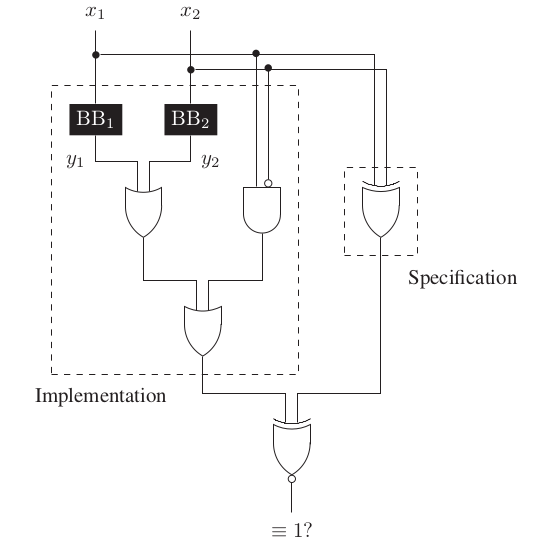
\includegraphics[width=9cm, height=7cm]{pec}
	\centering
	\caption{PEC}\label{fig:pec}
\end{figure}

\begin{example} \label{eg:dqbf}
Consider $x_1 \oplus x_2$ as the specification and as an
implementation a partial circuit with three gates and two black boxes as given in Fig.~\ref{fig:pec}.
PEC problem: Is there a realization of both black boxes $BB_1$ and $BB_2$ such that the implementation is equivalent to the specification for every value of the inputs $x_1$ and $x_2$?

To answer this question, we add an additional equivalence (or XNOR) gate for each corresponding output of the specification and implementation and require the outputs of these equivalence gates to be constantly 1.
\end{example}

\subsubsection{DQBF formulation}\label{sssec:dqbf-fml}
Both \cite{gitinarswb13, gitinarswb13r} present a linear transformation from PEC to DQBF such that the resulting DQBF is satisfied if and only if the PEC is realizable.

Let's introduce notations for partial combinational circuits $P$ :

\begin{itemize}
\item $x_1,\dots,x_n$: primary inputs of the circuit.
\item $BB_1 ,\dots, BB_m$: black boxes of the circuit in topological order.
\item $\overrightarrow{I_i}$: inputs of $BB_i (i = 1,\dots, m)$.
\item $\overrightarrow{Y_i}$: inputs of $BB_i (i = 1,\dots, m)$.
\item $\overrightarrow{F_i}(x_1,\dots, x_n, Y_1,\dots,Y_{i-1}$: vector of functions defining $\overrightarrow{I_i}$.
\item $R(x_1,\dots, x_n, Y_1,\dots,Y_{m}$: is the output function of the circuit.
\end{itemize}
\begin{figure}[]
	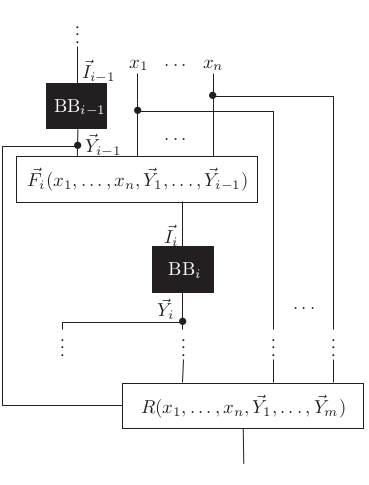
\includegraphics[width=6cm, height=7cm]{not}
	\centering
	\caption{PEC}\label{fig:notation}
\end{figure}

We assume w.l.o.g. that $Y_i \cap I_j = \emptyset$  for all $i,j$. That means no output of a black box is directly connected to an input of another black box.
The primary inputs $x_1 ,\dots, x_n$ and the black box inputs $\overrightarrow{I_1},\dots,\overrightarrow{I_m}$ are universally quantified, all other variables are existentially
quantified.
The dependency set of black box output $y_{i,j}$ contains exactly the inputs $\overrightarrow{I_i}$ of $BB_i$.
We construct the quantifier prefix of the DQBF as follows:
\[
\forall x_1,\dots,x_n \, \forall \overrightarrow{I_1},\dots,\overrightarrow{I_m} \, \exists \overrightarrow{Y_1}(\overrightarrow{I_1}),\dots, \exists \overrightarrow{Y_m}(\overrightarrow{I_m})
\]
If the black boxes are not directly connected to the primary inputs but to internal signals we have to take into account that not all possible combinations of values may arrive at the inputs of the black boxes.
Since we use a universal quantification for the black box inputs we have to ensure that our formula is satisfied if the value of the black box inputs $I_i$ deviates from the values
obtained as a function $\overrightarrow{F_i} (x_1 ,\dots, x_n,\overrightarrow{Y_1} ,\dots ,\overrightarrow{Y}_{i-1} )$

\begin{equation}
\begin{split}\nonumber
	 \varphi &=  \big( \overrightarrow{I_1} \not\equiv \overrightarrow{F_1} (x_1 ,\dots, x_n)  \big) \, \lor \, \dots \lor  \\
	 & \big( \overrightarrow{I_m} \not\equiv \overrightarrow{F_m} (x_1 ,\dots,x_m, \overrightarrow{Y_1} ,\dots,\overrightarrow{Y}_{m-1})  \big) \\
	 & \lor R(x_1,\dots, x_n, \overrightarrow{Y_1},\dots,\overrightarrow{Y_m})
\end{split}
\end{equation}

This formula is not necessarily given in CNF. By applying Tseitin transformation (introducing auxiliary variables for the internal signals of the circuit), one can obtain a
CNF $\varphi^{\prime}$ that is satisfiability equivalent to $\varphi$ and whose size is linear in the size of $\varphi$.
Let $\overrightarrow{A}$ be the vector of these auxiliary variables, which are existentially quantified in the quantifier prefix.
Their dependency set encompasses all universally quantified variables.

\begin{equation}
\begin{split}\nonumber
\Phi &= 	\forall x_1,\dots,x_n \, \forall \overrightarrow{I_1},\dots,\overrightarrow{I_m} \, \exists \overrightarrow{Y_1}(\overrightarrow{I_1}),\dots, \exists \overrightarrow{Y_m}(\overrightarrow{I_m}) \, \\
& \,\,\,\,\,\,\,\, \exists \overrightarrow{A}(x_1,\dots,x_n, \overrightarrow{I_1},\dots,\overrightarrow{I_m}): \varphi^{\prime}
\end{split}
\end{equation}

The formula $\Phi$ is satisfied if and only if we can replace
all $\overrightarrow{Y_i}$ with Skolem functions $\overrightarrow{s}_{\overrightarrow{Y_i},\overrightarrow{I_i}}$ such that $\varphi^{\prime}$ becomes a tautology.
The Skolem functions $\overrightarrow{s}_{\overrightarrow{Y_i},\overrightarrow{I_i}}$ exist if and only if there are implementations for the black boxes $BB_i$ of the PEC, such that the specification is realized.

\begin{lemma}
  Any PEC can be translated into an equivalent DQBF with linear effort.
\end{lemma}


\begin{example}
  For the Example~\ref{eg:dqbf} PEC can be translated to the following DQBF:
\begin{equation} \nonumber
  \Phi_{DQBF} = \forall x_1 x_2 \exists y_1 (x_1) y_2 (x_2) :
  \big( (y_1 \lor y_2) \lor (x_1 \land \neg x_2) \big) \equiv (x_1 \oplus x_2)
\end{equation}
The primary inputs $x_1$ and $x_2$ get universally quantified.
The input functions $F_1$ and $F_2$ are the identity functions (of $x_1$ and $x_2$).
The black box inputs are directly connected to the primary inputs and therefore we do not need additional variables for them.
The black box outputs $y_1$ and $y_2$ are existentially quantified.
The signal $y_1$ depends on $x_1$ ($BB_1$ has $x_1$ as input) and signal $y_2$ depends on $x_2$.
The three gates of the implementation (Example~\ref{eg:dqbf}) are represented by the Boolean expression $(y_1 \lor y_2) \lor (x_1 \land \neg x_2)$.
For the matrix (given the inputs of the black boxes are consistently assigned) we require the implementation must be equal to $(x_1 \oplus x_2)$.
\end{example}

\begin{lemma}
  Any DQBF can be translated into an equivalent PEC with linear effort (easy to show).
\end{lemma}

\begin{theorem}
  PEC and DQBF are polynomially equivalent.
\end{theorem}

\begin{corollary}
  PEC is NEXPTIME-complete.
\end{corollary}

\subsubsection{BMC for Incomplete Designs \cite{drechsler2018formal}}
The complexity of deciding realizability depends on the allowed behavior of the black boxes:
\begin{enumerate}
  \item If we assume that the contents of the black boxes are combinational circuits, the problem of deciding realizability is NEXPTIME-complete.
  \item If we allow the black boxes to contain an arbitrary amount of memory, the interesting decision problems become undecidable \cite{pnuelir90}.
\end{enumerate}

Bounded Model Checking (BMC) for incomplete design was studied in \cite{millerklb10, millersb13}. Only invariant
properties were considered: Given a Boolean formula $P(x, s, y)$, which describes the states of the circuit that satisfy the invariant, are there implementations of the black boxes such that $P(x, s, y)$ is satisfied in each step of the circuit?

First a QBF modeling was presented. However, if the black box in the design is not directly connected to all primary inputs, (i.e., if the black box does not have ``complete information"), the property may be unrealizable, although BMC with QBF modeling is not able to prove this.
In that case, DQBF is necessary to express the actual dependencies of the black boxes on their inputs.
XXX

\subsection{Distributed Synthesis for LTL Fragments \cite{chatterjee13}}

%\cite{chatterjee13} consider the distributed synthesis problem for temporal logic specifications.

The distributed synthesis problem \cite{pnueli90} extends
the classical synthesis problem of constructing a system from a given temporal logic specification to a distributed setting.

The input for distributed synthesis problem is:
\begin{enumerate}
  \item An architecture of synchronously communicating processes, that exchange messages through communication channels.
  \item A specification given as a temporal logic formula.
\end{enumerate}

The synthesis question is: to construct a reactive system for each process such that the specification is satisfied.
The logic used to express the temporal logic specification is the linear-time temporal logic (LTL).

Previous results:
In general the distributed synthesis problem is undecidable for LTL, but the problem is decidable for pipeline architectures.
The undecidability proof uses ideas originating from the undecidability proof of three-player imperfect-information games \cite{peterson2001lower}.

The result of the paper relevant to us: Temporal specifications without the next operator (a fragment of LTL, LTL$_{AG}$) is NEXPTIME-complete.
%The problem of realizability is decidable in non-deterministic exponential time in the size of the specification.
If we consider a set of safety assumptions, and a set of guarantees such that each guarantee is a safety, reachability, or a liveness guarantee, then the distributed synthesis problem is NEXPTIME-complete for all architectures.

Fragment LTL$_{AG}$. Consider formulae $\phi$ from the following LTL fragment (standard semantics of LTL is used: $\square$ is Globally; property is always true. $\lozenge$ is Finally: property eventually has to hold ):

\begin{flalign*}
  \phi &= \bigwedge_i \square P_i \to \big( \bigwedge_i \square Q_i \land \bigwedge_i \square \lozenge R_i \land \bigwedge_i \lozenge F_i \big)
\end{flalign*}

for $i \in {1,\dots,m}$, with $P_i$,
$Q_i$, $R_i$, $F_i$ are propositional formulae, P = $\land_i P$ and Q = $\land_i Q$.
This fragment can express specifications that
consist of conjunction of safety assumptions, and guarantees
where each guarantee is a safety, reachability, or a liveness
condition.

Local strategy: For every process $p$ a local strategy is a function setting the output variables of $p$ according to the history of its input variables. They only depend on the
information available.

Memoryless strategy: they do not depend on the
history, only on the current state.

\begin{lemma}
  Deciding whether every $\phi_{F_i}, \phi_{R_i}$ is realizable reduces to realizing the propositional formulae $(P \to (Q  \land R_i))$ and $(P \to (Q  \land F_i))$.
\end{lemma}

\begin{lemma}
  Every formula $ \phi \in LTL_{AG}$ is realizable if and only if it admits local strategies for all the corresponding $\phi_{F_i}, \phi_{R_i}$
\end{lemma}

Deciding whether every $\phi_{F_i}, \phi_{R_i}$ is realizable can be done in NEXPTIME, by having a non-deterministic Turing machine guessing the local strategies of all processes, and verifying that such strategies satisfy the formula under all the (exponentially many) possible inputs of the environment.

The problem is shown to be NEXPTIME-hard, via a reduction
from the Dependency Quantifier Boolean Formula (DQBF)
validity problem \cite{peterson2001lower}.

\begin{theorem}
  Given an architecture $A$ and a formula  $\phi \in LTL_{AG}$,
  deciding whether $\phi$ is realizable in $A$ is NEXPTIME-hard.
\end{theorem}

\begin{theorem}
  Given an architecture $A$ and a specification $\phi \in LTL_{AG}$, the realizability of $\phi$ in A is NEXPTIME-complete.
\end{theorem}

\section{First solving approach: DQDPLL}
The first solving approach was presented in~\cite{frohlich2012dpll}.
%
This was adaptation of QDPLL from QBF to DQBF, e.g., unit propagation, clause
learning, universal reduction, watched literals, etc.
%

The motivation was to solve the quantifier-free bit-vector formulas (QF\_BV) by translating it to DQBF (both belongs to same complexity class).
%
The presented algorithm solve DQBF based on variable elimination (\cite{biere2004resolve}).

\section{First publicly available solver}
The technique presented in~\cite{finkbeiner2014fast} is similar to BMC encoding of QBF and can only solve UNSAT problems.

\section{Complete solver: iDQ}
The iDQ solver presented in~\cite{frohlich2014idq} adapts and extends the Inst-Gen approach (solving approach for EPR logic, fragment of first order logic) to DQBF.

\section{A new solver: HQS}
The work of~\cite{gitina2015solving} present an improved expansion-based solver, HQS.
%
The solver expands DQBF to QBF, eliminates the minimum set of variables that cause non-linear
dependencies and uses AIGs to detect units and pure literals.

\section{Preprocessing and inprocessing}
The work of~\cite{wimmer2015preprocessing} generalize preprocessing techniques for QBF to DQBF.
%
The technique includes, blocked clause elimination, equivalence reasoning, structure extraction, and variable elimination by resolution.

In further work~\cite{wimmer2017hqspre} presents a preprocessor HQSpre for both QBF's and DQBF's.
%
The techniques, variable elimination routines, clause elimination routines, clause strengthening routines, dependency schemes and gate rewriting.

\section{Dependency}
The work by~\cite{wimmer2016dependency} analyse the dependency
schemes proposed for QBF to apply on DQBF.
%
The paper gives correctness proof of the few that are sound for DQBF.
%

The \cite{wimmer2017dqbf} eliminate of dependencies of DQBF to convert it to an equisatisfiable QBF.
%
The technique is implemented in HQS.

% which result from the application of dependency schemes to the formula and can be added to or removed from the formula at no cost


The work ~\cite{beyersdorff2018reinterpreting} proposed an approach which improve the relationship between DQBF and QBF
dependency schemes.
%
Core of the paper is the method that gives rise to soundness results across different calculi.

\section{Proof systems}
The work~\cite{beyersdorff2016lifting} examines the lifting existing resolution systems of QBF to DQBF.
%
QBF have a strict chain of proof systems, where Q-Res $<$ IR-calc $<$ IRM-calc.
%

In the case of DQBF the obvious adaptations of Q-Res and universal resolution turns out to be too weak: they are not complete.
%
The obvious adaptation of IR-calc has
the right strength: it is sound and complete.
%
The IRM-calc and long-distance resolution is too strong: it is not sound any more.

The work of~\cite{rabe2017resolution} presents a sound and complete proof system for DQBF.
%
The system has three rules, resolution, universal reduction, and a new proof rule called \textit{fork extensions}.

The definition of resolution admits universal variables as pivots\dots

\section{Certification perspective and Skolem functions}

%\begin{enumerate}
The work of Henkin Quantifiers and Boolean Formulae~\cite{balabanov2012henkin} investigates DQBF's properties like negation, complement, formula expansion, and prenex, non-prenex form conversion.
%
The paper used two forms to describe prenex DQBF, Skolem (S-Form) and Herbrand (H-Form) form:

\begin{align}
\Phi_{S} \,\, = \,\, \forall x_{1}\dots \forall x_{n} \exists y_{1_{(S_{1})}}\dots\exists y_{m_{(S_{m})}} . \phi \label{eq1}\\
\Phi_{H}  \,\, = \,\, \forall x_{1_{(H_{1})}}\dots \forall x_{n_{(H_{n})}} \exists y_{1}\dots\exists y_{m} . \phi \label{eq2}
\end{align}

Additional subscripts on the quantified variables is just another way to express dependencies, $S_{i} \subseteq A$ and $H_{i} \subseteq E$.

In the case of S-Form, $\exists y_{1_{(S_{1})}}$ means  existential variable $y_{1}$ depend on the universal variables set $S_{1}$.
%
Similarly, for the H-form, universal quantifiers in the prefix are annotated with the existential variables they depend on.

%Semantically, the truth and falsity of a DQBF is interpreted as existence of Skolem (in the case of \ref{eq1}) and Herbrand fucntion (in the case of \ref{eq2}).
Skolem functions serve as the model to a true S-form DQBF whereas Herbrand functions serve as the countermodel to a false H-form DQBF.

Most important property discussed is the notion of \textbf{negation} and \textbf{complement}.
%
In the case of negation ($\neg$) the quantifiers are flipped and propositional formula is negated but no change in the dependency set and it's position.

\begin{align}
\neg \Phi_{S} \,\, =   \,\, \exists x_{1}\dots \exists x_{n} \forall y_{1_{(S_{1})}}\dots\forall y_{m_{(S_{m})}} . \neg \phi \label{eq3}
\end{align}

In the case of complement ($\sim$) the position is shifted from one quantifier type to another in the prefix. Here, $H^{\prime}_{i} = \{ y_{i} \in E \, | \, x_{i} \notin S_{j} \}$

\begin{align}
\sim \Phi_{S} \,\, =   \,\, \exists x_{1_{(H^{\prime}_1)}}\dots \exists x_{1_{(H^{\prime}_n)}} \forall y_{1}\dots\forall y_{m} . \neg \phi \label{eq4}
\end{align}

Interestingly the following proposition holds,
\begin{prop}
	DQBF under the negation operation obeys the law of excluded middle but under the complement operation it does not.
\end{prop}

In the journal paper ``A certification perspective of DQBF"~\cite{balabanov2014henkin} additionally a generalized resolution rule for DQBF evaluation is presented. Although,  it is shown to be sound, but incomplete.

Two central references in both are~\cite{bubeck2006dependency} and ~\cite{bubeck2010model} in introduction section referring that S-form DQBF can be converted to an equivalent QBF by formula expansion on the universal variables.

%\end{enumerate}

The work by~\cite{wimmer2016skolem} obtains Skolem functions from an elimination-based DQBF solver HQS, while taking preprocessing steps into account.
%
The size of the Skolem functions is optimized by don’t-care minimization using Craig interpolants and rewriting techniques.


\section{Experiments}\label{sec:experiments}
We perform two sets of experiments. Finding autarkies on the selected benchmarks and evaluating the effect of the autarky-reduction on a particular solver.

We performed autarky search experiments on benchmarks from both the DQBF- (334 instances) and  PCNF-track (463 instances) of QBFEVAL'18 \cite{Qbfeval18}.
%
From the QBFLIB benchmark \cite{Qbflib}, we removed non-PCNF instances (instances in qcir format) and selected instances in PCNF format (25,522 instances) for the experiment.

% We also performed autarky search experiments on  PCNF format (25,650 instances) instances of .
%QBFEVAL'18 benchmarks (total 1234 instances) and .

%From the QBFEVAL'18 benchmarks \cite{Qbfeval18}, we selected instances in PCNF format and removed non-PCNF instances (instances from QCIR-track). In total, we considered 334 instances from DQBF-track and 463 instances from PCNF-track.
%Similarly, from QBFLIB benchmarks \cite{Qbflib} we removed all instances that are not in PCNF. In total, we considered 25,650 instances from QBFLIB to perform the autarky search.

We selected four (D)QBF solvers to perform the evaluation of autarky-reduction. Top three solvers of QBFEVAL'19 PCNF-track competition; \caqe \cite{DBLP:conf/fmcad/RabeT15}, \depqbf \cite{DBLP:conf/cade/LonsingE17}, \qute \cite{DBLP:journals/jsat/PeitlSS19}\ and the winner of DQBF-track competition, \hqspre \cite{DBLP:conf/tacas/WimmerRM017}.

All the experiments were performed on our cluster where each compute node has
two Intel Xeon E5-2620 v4 CPUs running at 2.10 GHz with turbo-mode disabled.
Time limit was set to 2700 seconds and memory limit to 7 GB.

\subsection{Implementation}
We have implemented the translation for $\Aaut_1$- and $\Eaut_1$-autarky search  (\ref{sec:a1-translation}, \ref{sec:e1-translation}) in a small codebase \autfinder\footnote{https://github.com/arey0pushpa/dcnf-autarky}. The \autfinder\ includes 2,000 lines of C++ code.

The translation requires for each $v \in E$ expressing AMO constraints in equation~\ref{eq:transAMO}, we implemented three encodings, binomial, logarithmic and linear. One of these options can be selected with the $\Aaut_1$ or $\Eaut_1+\Aaut_1$ autarky type. The resulted CNF formula is solved by the lingeling \cite{Biere-SAT-Competition-2017-solvers} SAT solver.


\begin{table}
\caption{Families of (D)QCNF instances and the corresponding autarky count}\label{tab:aut-count}
\begin{tabular}{c|l|c|c|c|c}

\hline
   \multirow{2}{1cm}{Sr.No} &  \multirow{2}{3cm}{Family} &  \multirow{2}{2cm}{Total instances} & \multicolumn{3}{c}{Autarky system} \\
    % \hline
    % \textbf{Inactive Modes} & \textbf{Description}\\
    \cline{4-6}
  & & & E1-Autarky & A1-Autarky & E1+A1-Autarky \\
    %\hhline{~--}

\hline

1. & DQBF-track'19 &  334 & 20 & 22 & 22[1] \\ \hline
%2. & PCNF-track'19 &  463 & 186 & 48[3] & 194[4] \\ \hline
2. & PCNF-track'19 &  559 & 200 & 40[4] & 50[6] \\ \hline
% Doable Small+ Low Autarky
3. & Akshay-Chakraborty-J-S-R &  44 & 42 & 4[3] & 44[3] \\ \hline
% No E1, small+medium in size
4. & Amendola-Ricca-Truszczynski & 1933 & &  &  \\ \hline

%% No E1 Check, medium in size
5. & Ansotegui &  38 & &  &  \\ \hline

% Medium (Very big and few small) Low Autarky, choti choti
6. & Ayari &  71 &  &  &  \\ \hline

% Small +, Low Autarky
7. & Basler &  713 & & &  \\ \hline

%% No E1 Check, Small + to medium!
8. & Biere &  738 & &  &  \\ \hline

% YUGEEE but some Autarky
9. & Cashmore-Fox-Giunchiglia &  150 &  &  &  \\ \hline

%% No History Check: Very SMALL TARGET!!, Complete E 1 and A1 bith
10. & Castellini &  169 & &  &  \\ \hline

%% No E1 Check Small +m Complete the E1 redution run
11. & Chen &  200 &  &  &  \\ \hline

% No E1 Check Small _ Medium
12. & Diptarama-Jordan-Shinohara &  180 &  &  &  \\ \hline

% No history Check Small TARGET, Run E1
13. & Egly-Seidl-Tompits-Woltran-Zolda &  1080 &  &  &  \\ \hline

% No History Check Medium, Run E1
14. & Faber-Leone-Maratea-Ricca &  1060 &  &  &  \\ \hline

% Big but have some autarkies
15. & Gent-Rowley &  672 &  &  &  \\ \hline

% Medium Big Small Combination but have some autarkies
16. & Herbstritt &  478 & &  &  \\ \hline

17. & Jordan-Kaiser &  4608 & &  &  \\\hline

%% No  E1 Check Small +
18. & Katz &  20 &  &  &  \\ \hline

% No E1 Check Small
19. & Klieber & 50 &  &  &  \\ \hline

% Small Good Autarkies E1 not A1 TARGET!
20. & Kontchakov&  136 & &  &  \\ \hline

% BIg Excelelnt Autarkies E1
21. & Kronegger-Pfandler-Pichler &  1700 &  &   & \\ \hline

% No E1 Check Small
22. & Lahiri-Seshia & 3 & &  &  \\ \hline

% No E1 Check  Medium
23. & Lee-Jiang &  5 &  &  &  \\ \hline

% SAT :) Check!!
24. & Letz & 14 &  &  &  \\\hline

% Small :) No E1
25. & Ling &  8 & &  &  \\ \hline

% Yuge low Autarky
26. & Mangassarian-Veneris &  171 & &  &  \\ \hline

%% Small+ low Autarky Target
27. & MayerEichberger-Saffidine &  312 & & & \\\hline

%%Small to big, No E1!
28. & Messinger &  63 & &  &  \\ \hline

%%Small to medium, Low autakr
29. & Miller-Marin & 2632 & &  &  \\ \hline

30. & Miller-Scholl & 198 & &  &  \\ \hline

%%Small to big, Low Autarky, Check again E1
31. & Mneimneh-Sakallah &  202 & &  &  \\ \hline

% Medium but too many Can Skip this Family!! No E1!
32. & Narizzano &  4000 & &  &  \\ \hline

% small a few rest BIG , No E1!
33. & Palacios & 24 &  &  &  \\ \hline

% Small target!! No E1!  Medium
34. & Pan &  384 & &  &  \\ \hline

% No E1, Small check A1
35. & Peitl & 10 &  &  &  \\\hline

% Small to medium, Low Autarkies
36. & qbfeval12 & 17 & &  &  \\ \hline

% Mediumbut have low autarkies
37. & Rabe &  17 &  & &  \\ \hline

% Small + size, Small Autarkies
38. & Rintanen &  131 & &  &  \\\hline

%% Medium to Big (a few small), Low Autarky
39. & Sauer-Reimer &  928 & &  & \\ \hline

% Check Small, low autarky, Recalculate some changes/
40. & Scholl-Becker & 64 &  &  &  \\ \hline

% medium, Low Autarkies
41. & Seidl &  200 &  &  &  \\ \hline

% Some SAT Some RED!! Small, recheck E1
42. & Tacchella &  336 & &  &  \\ \hline

% Big Medium, No E1
43. & Tentrup & 1354 &  &  &  \\ \hline \hline

Total &  & 26010 &  &  &  \\  \hline \hline


\hline
\end{tabular}
\end{table}


\subsection{Results}
We use the name of the author to refer to the submitted families of the benchmarks. This is the structure the QBFLIB is organised.

In Table~\ref{tab:aut-count} we present the complete results of the autarky search. For example, out of 334 instances in the DQBF track of QBFEVAL'18, 330 instances are $\Eaut_1+\Aaut_1$-lean (have no non-trivial $\Eaut_1$- or $\Aaut_1$-autarky). From the remaining 4 instances, all are $\Eaut_1$-lean, one is $\Aaut_1$ satisfiable, one is $\Eaut_1+\Aaut_1$ satisfiable, and the remaining two instances are not $\Eaut_1+\Aaut_1$ satisfiable, but allow $\Aaut_1$-autarkies elimination.
%
There are a few families of the benchmarks like \textit{Castellini} that has a healthy number of autarkies of all types, $\Eaut_1,\Aaut_1,\Eaut_1+\Aaut_1$. On the other hand there are families like \textit{Tentrup} and  with no autarkies at all. There are total 714 (autarky satisfiable) instances which can be directly solved as a part of autarky cleanup.
% in both cases around 70\% of variables and clauses (while adding E1 does not change this).

Table~\ref{tab:sat-solver} shows the number of $\Eaut_1+\Aaut_1$-autark-SAT instance solved by the corresponding (D)QCNF solvers. There are a few instances that are autarky-satisfiable but the solver was unable to solve them in the given time. In particular there was a large set of trivially satisfiable autarky instances which \hqspre\ was unable to solve. This is relevant to our case as our focus is primarily DQCNF and provide a hint that $\Eaut_1+\Aaut_1$ autarky search is not already covered by other pre-processing techniques.

Next out of the total 10,708 autarky instances we select at random around 1100 instances to register the effect of the autarky reduction on the solvers. The selection
%
%Out of total 463 instances of the PCNF-track of QBFEval'18 we found that 269 instances are $\Eaut_1+\Aaut_1$ Lean.
Table~\ref{tab:solver-eval} present the result of solver running on the original instance vs on the autarky-reduced instance. We found XXX

%We randomly sample from the set of autarky-reduced instances. To represent each family of benchmarks evenly, we normalise the selection. We take the relative contribution of each family to the total number of 2,000 autarky-reduced instances. XXX


\begin{table}
	\caption{Total $\Eaut_1+\Aaut_1$ Autark-SAT instance solved by the corresponding (D)QCNF solvers}\label{tab:sat-solver}
	\begin{tabular}{l|c|c|c|c}

		\hline
		\multirow{2}{3cm}{Family}  & \multicolumn{4}{c}{(D)QCNF Solver} \\
		% \hline
		% \textbf{Inactive Modes} & \textbf{Description}\\
		\cline{2-5}
		& Caqe & DepQbf & Qute & HQSpre  \\
		%\hhline{~--}

		\hline

		SAT-instances (500) &  474 & 484 & 485 & 392 \\

		\hline
	\end{tabular}
\end{table}

\begin{table}
	\caption{Comparison of the (D)QCNF instances solved without and with autarky reduction. \emph{Orig} represent the original instance and \emph{Red} represent the autarky reduced formula. Number inside () represents uniquely solved instances.  }\label{tab:solver-eval}
	\begin{tabular}{l| c |c c c }

		\hline
		\multirow{2}{2.5cm}{Solvers} &  \multirow{2}{1cm}{Type} & \multicolumn{3}{c}{Instances} \\
		\cline{3-5}
		& & Random-255 [$\Aaut_1$] & Random-336 [$\Eaut_1+\Aaut_1$] & Random-500 [$\Eaut_1$] \\\hline
		% \hline
		% \textbf{Inactive Modes} & \textbf{Description}\\

		%   & & \multicolumn{2}{c}{Caqe} &\multicolumn{2}{c}{Depqbf} & \multicolumn{2}{c}{Qute}& \multicolumn{2}{c}{HQSpre}\\  \cline{3-10}
		%     & & Orig & Red & Orig & Red & Orig & Red & Orig & Red \\
		%\hhline{~--}

		\hline
		\multirow{2}{*}{\caqe} & Orig & 193(4) & 228(2) & 381(2) \\
		& Red & 196(7) & 230(4) & 380(1)\\\hline
		\multirow{2}{*}{\depqbf} & Orig & 184(2) & 231(1) & 365(7)\\
		& Red & 183(1)& 232(2)& 367(9)\\\hline
		\multirow{2}{*}{\qute} & Orig & 117(1) & 205(0) & 283(3)  \\
		& Red  & 124(8) & 210(5) & 281(1) \\\hline
		\multirow{2}{*}{\hqspre} & Orig & 96(0) &251(0) & 279(4) \\
		& Red  & 98(2)& 254(4) & 280(5) \\
		% &
		%Qute &
		%HQSpe &
		%Random set-1 &  326 & 228(2) & 230(4) & 231(1) & 232(2) & 205(0) & 210(5) & 251(0)& 254(4) \\ \hline
		%%PCNF-track'18 &  463 & 168 & 82 & 174 \\ \hline
		%Random set-2 ($\Eaut_1+\Aaut_1$)&  255 & 193(4) & 196(7) & 184(2)& 183(1) & 117(1) & 124(8) & 96(0)& 98(2) \\\hline
		%Random set-3 (Only E1) &  500 & 381(2) & 380(1) & 365(7) & 367(9) & 283(3) & 281(1) & 279(4) & 280(5) \\

		\hline
	\end{tabular}
\end{table}

\section{Conclusion}
\label{sec:conclusion}

\bibliographystyle{apalike}
\bibliography{DQBF_Autarky}

\end{document}

%%% Local Variables:
%%% mode: latex
%%% TeX-master: t
%%% End:
